\documentclass[12pt]{article}
\usepackage{hyperref}
\usepackage{amsmath,amsfonts,amssymb}
\usepackage{fullpage}
\usepackage{xcolor}
\usepackage{enumitem}
\usepackage{booktabs}
\usepackage{tikz}
\usetikzlibrary{arrows.meta,decorations.pathmorphing,decorations.markings,calc}

\hypersetup{
    colorlinks=true,
    linkcolor=blue!70!black,
    citecolor=blue!70!black,
    urlcolor=blue!70!black
}

\newcommand{\be}{\begin{equation}}
\newcommand{\ee}{\end{equation}}
\newcommand{\bh}{\bar{h}}

\newcounter{quesno}
\newcommand{\ques}[2]{%
  \ifnum\thequesno>0 \clearpage \fi
  \stepcounter{quesno}%
  \noindent\rule{\textwidth}{1.0pt}\vspace{0.4em}\par
  \noindent{\bfseries\Large Question \thequesno.} \emph{(#1 points)}\par\vspace{0.6em}
  \noindent{\itshape #2}\par\vspace{0.8em}
  \noindent\rule{\textwidth}{0.4pt}\vspace{0.6em}\par
  \noindent{\bfseries\large Solution:}\par\vspace{0.5em}
}

\begin{document}

\begin{center}
{\bf\LARGE General Relativity}\\[0.6em]
{\bf\Large Final Examination --- Comprehensive Model Solutions}\\[0.6em]
\end{center}

\vspace{0.3em}
\hrule height 1.2pt
\vspace{0.8em}
\noindent
{\bf Instructions Reference:} All questions are answered below in full detail, presenting every necessary intermediate calculational step, tensor transformation, metric derivation, and physical discussion required for complete marks.
\vspace{0.5em}
\hrule
\vspace{0.5em}

% =========================================================================
% QUESTION 1
% =========================================================================
\ques{2}{%
The components of the Riemann tensor in some coordinates are $R^\mu{}_{\nu\rho\sigma}$.
Write down how they transform under a change of coordinates.
Define the Ricci tensor by $R_{\mu\nu} = R^\rho{}_{\mu\rho\nu}$, and show explicitly that this transforms as a tensor under change of coordinates.
}

\subsection*{1. Transformation of the Riemann Tensor}

Let $x^\mu$ denote the coordinates of an event in a chart on a smooth manifold $M$, and let $x'^\alpha$ denote the coordinates of the same event in another chart under a smooth, invertible coordinate transformation $x \mapsto x'(x)$. 
The transition matrices (Jacobian matrix and its inverse) between the two coordinate charts are defined by:
\be
\Lambda^\alpha{}_\mu \equiv \frac{\partial x'^\alpha}{\partial x^\mu} \,, \qquad 
(\Lambda^{-1})^\mu{}_\alpha \equiv \frac{\partial x^\mu}{\partial x'^\alpha} \,.
\ee
By the multivariable chain rule, these Jacobian matrices satisfy the standard inverse completeness and orthogonality relations:
\be
\frac{\partial x'^\alpha}{\partial x^\mu} \frac{\partial x^\mu}{\partial x'^\beta} = \delta^\alpha_\beta \,, \qquad
\frac{\partial x^\mu}{\partial x'^\alpha} \frac{\partial x'^\alpha}{\partial x^\nu} = \delta^\mu_\nu \,.
\label{eq:jac_inv}
\ee
The Riemann curvature tensor is a $(1,3)$ tensor (possessing one contravariant index and three covariant indices). Under the coordinate transformation $x \to x'$, its components transform multilinearly according to:
\be
R'^\alpha{}_{\beta\gamma\delta} = \frac{\partial x'^\alpha}{\partial x^\mu} \frac{\partial x^\nu}{\partial x'^\beta} \frac{\partial x^\rho}{\partial x'^\gamma} \frac{\partial x^\sigma}{\partial x'^\delta} R^\mu{}_{\nu\rho\sigma} \,.
\label{eq:riemann_transf}
\ee
Here, the upper index transforms with the forward Jacobian $\frac{\partial x'^\alpha}{\partial x^\mu}$, while each of the three lower indices transforms with the inverse Jacobian $\frac{\partial x^\nu}{\partial x'^\beta}$, $\frac{\partial x^\rho}{\partial x'^\gamma}$, and $\frac{\partial x^\sigma}{\partial x'^\delta}$.

\subsection*{2. Definition and Tensor Transformation of the Ricci Tensor}

The Ricci curvature tensor $R_{\mu\nu}$ is defined by contracting the upper contravariant index of the Riemann curvature tensor with its second lower covariant index:
\be
R_{\mu\nu} \equiv R^\rho{}_{\mu\rho\nu} \,.
\label{eq:ricci_def}
\ee
In the primed coordinate system $x'$, the components of the Ricci tensor are given by the identical contraction of the primed Riemann tensor components:
\be
R'_{\beta\delta} \equiv R'^\alpha{}_{\beta\alpha\delta} \,.
\label{eq:ricci_primed_def}
\ee
To demonstrate explicitly that $R_{\mu\nu}$ transforms as a $(0,2)$ tensor, we substitute the general Riemann tensor transformation law \eqref{eq:riemann_transf} into the definition of $R'_{\beta\delta}$ \eqref{eq:ricci_primed_def}, setting both the contravariant index and the second covariant index to the summation index $\alpha$:
\be
R'_{\beta\delta} = \frac{\partial x'^\alpha}{\partial x^\mu} \frac{\partial x^\nu}{\partial x'^\beta} \frac{\partial x^\rho}{\partial x'^\alpha} \frac{\partial x^\sigma}{\partial x'^\delta} R^\mu{}_{\nu\rho\sigma} \,.
\ee
Since the partial derivatives are ordinary functions that commute under multiplication, we can reorder the terms so that the two Jacobian factors carrying the contracted index $\alpha$ are grouped together:
\be
R'_{\beta\delta} = \left( \frac{\partial x'^\alpha}{\partial x^\mu} \frac{\partial x^\rho}{\partial x'^\alpha} \right) \frac{\partial x^\nu}{\partial x'^\beta} \frac{\partial x^\sigma}{\partial x'^\delta} R^\mu{}_{\nu\rho\sigma} \,.
\ee
Applying the chain rule relation from equation \eqref{eq:jac_inv}:
\be
\frac{\partial x'^\alpha}{\partial x^\mu} \frac{\partial x^\rho}{\partial x'^\alpha} = \frac{\partial x^\rho}{\partial x^\mu} = \delta^\rho_\mu \,.
\ee
Substituting this Kronecker delta into our expression for $R'_{\beta\delta}$:
\be
R'_{\beta\delta} = \delta^\rho_\mu \frac{\partial x^\nu}{\partial x'^\beta} \frac{\partial x^\sigma}{\partial x'^\delta} R^\mu{}_{\nu\rho\sigma} \,.
\ee
We now execute the contraction over the dummy index $\mu$ using the Kronecker delta $\delta^\rho_\mu$:
\be
\delta^\rho_\mu R^\mu{}_{\nu\rho\sigma} = R^\rho{}_{\nu\rho\sigma} \,.
\ee
According to the original definition \eqref{eq:ricci_def} of the Ricci tensor in the unprimed coordinate chart, this contracted object is precisely the unprimed Ricci tensor component $R_{\nu\sigma}$:
\be
R^\rho{}_{\nu\rho\sigma} = R_{\nu\sigma} \,.
\ee
Therefore, we obtain:
\be
R'_{\beta\delta} = \frac{\partial x^\nu}{\partial x'^\beta} \frac{\partial x^\sigma}{\partial x'^\delta} R_{\nu\sigma} \,.
\label{eq:ricci_transformed_final}
\ee
Relabeling the indices to standard modern notation ($x \to x'$, with indices $\mu,\nu \to \mu',\nu'$ and dummy indices $\rho,\sigma$):
\be
R'_{\mu'\nu'} = \frac{\partial x^\rho}{\partial x'^{\mu'}} \frac{\partial x^\sigma}{\partial x'^{\nu'}} R_{\rho\sigma} \,.
\ee
Equation \eqref{eq:ricci_transformed_final} is precisely the defining transformation law for a $(0,2)$ tensor (a rank-2 covariant tensor) under an arbitrary change of coordinates. 
This completes the explicit proof that the contraction of the Riemann tensor yielding the Ricci tensor is a tensor.

% =========================================================================
% QUESTION 2
% =========================================================================
\ques{3}{%
Consider a manifold on which we have both a metric, $g_{\mu\nu}$, and a totally antisymmetric $(0,3)$ tensor, $H_{\mu\nu\rho} = H_{[\mu\nu\rho]}$.
We can define a connection with components $\hat\Gamma_{\mu\nu}{}^\rho$ by:
\be
\hat \Gamma_{\mu\nu}{}^\rho = \Gamma_{\mu\nu}{}^\rho + \frac{1}{12} g^{\rho \sigma} H_{\mu\nu\sigma}
\label{eq:stringconn_q}
\ee
where $\Gamma_{\mu\nu}{}^\rho$ denotes the components of the usual Levi-Civita connection.

\begin{enumerate}[label=\alph*)]
\item (\emph{2 points}) Is the new connection $\hat\Gamma_{\mu\nu}{}^\rho$ defined in equation \eqref{eq:stringconn_q} torsion-free? Is it metric compatible? 
\item (\emph{1 point}) Show that the geodesics of the connection $\hat\Gamma_{\mu\nu}{}^\rho$ are the same as the geodesics of the Levi-Civita connection. 
\end{enumerate}
}

\subsection*{Part a) Torsion and Metric Compatibility}

\paragraph{1. Torsion Analysis:}
The torsion tensor $T^\rho{}_{\mu\nu}$ of a connection with components $\hat\Gamma_{\mu\nu}{}^\rho$ is defined as the antisymmetric part of the connection with respect to its lower two indices:
\be
T^\rho{}_{\mu\nu} \equiv \hat\Gamma_{\mu\nu}{}^\rho - \hat\Gamma_{\nu\mu}{}^\rho \,.
\label{eq:torsion_def}
\ee
Substituting the explicit definition of the connection \eqref{eq:stringconn_q} into equation \eqref{eq:torsion_def}:
\be
T^\rho{}_{\mu\nu} = \left( \Gamma_{\mu\nu}{}^\rho + \frac{1}{12} g^{\rho\sigma} H_{\mu\nu\sigma} \right) - \left( \Gamma_{\nu\mu}{}^\rho + \frac{1}{12} g^{\rho\sigma} H_{\nu\mu\sigma} \right) \,.
\ee
Because $\Gamma_{\mu\nu}{}^\rho$ is the standard Levi-Civita connection, it is torsion-free by definition, meaning its lower indices are completely symmetric:
\be
\Gamma_{\mu\nu}{}^\rho - \Gamma_{\nu\mu}{}^\rho = 0 \,.
\ee
The torsion tensor therefore simplifies to:
\be
T^\rho{}_{\mu\nu} = \frac{1}{12} g^{\rho\sigma} \left( H_{\mu\nu\sigma} - H_{\nu\mu\sigma} \right) \,.
\ee
We are given that $H_{\mu\nu\sigma}$ is a totally antisymmetric $(0,3)$ tensor ($H_{\mu\nu\sigma} = H_{[\mu\nu\sigma]}$). In particular, swapping its first two indices introduces a minus sign:
\be
H_{\nu\mu\sigma} = - H_{\mu\nu\sigma} \implies H_{\mu\nu\sigma} - H_{\nu\mu\sigma} = H_{\mu\nu\sigma} - (-H_{\mu\nu\sigma}) = 2 H_{\mu\nu\sigma} \,.
\ee
Substituting this into the torsion expression yields:
\be
T^\rho{}_{\mu\nu} = \frac{1}{12} g^{\rho\sigma} \left( 2 H_{\mu\nu\sigma} \right) = \frac{1}{6} g^{\rho\sigma} H_{\mu\nu\sigma} = \frac{1}{6} H_{\mu\nu}{}^\rho \,.
\ee
Since $H$ is a non-trivial totally antisymmetric tensor ($H \neq 0$), the torsion tensor does not vanish:
\be
T^\rho{}_{\mu\nu} \neq 0 \,.
\ee
\textbf{Conclusion on Torsion:} The new connection $\hat\Gamma_{\mu\nu}{}^\rho$ is \textbf{not} torsion-free. It has non-vanishing torsion $T^\rho{}_{\mu\nu} = \frac{1}{6} H_{\mu\nu}{}^\rho$.

\paragraph{2. Metric Compatibility Analysis:}
A connection $\hat\nabla$ is defined to be metric compatible if the covariant derivative of the metric tensor with respect to the connection vanishes identically:
\be
\hat\nabla_\lambda g_{\mu\nu} = 0 \,.
\ee
In components, the covariant derivative of a rank-2 covariant tensor under the connection $\hat\Gamma$ is:
\be
\hat\nabla_\lambda g_{\mu\nu} = \partial_\lambda g_{\mu\nu} - \hat\Gamma_{\lambda\mu}{}^\sigma g_{\sigma\nu} - \hat\Gamma_{\lambda\nu}{}^\sigma g_{\mu\sigma} \,.
\label{eq:cov_metric}
\ee
Substituting $\hat\Gamma_{\mu\nu}{}^\rho = \Gamma_{\mu\nu}{}^\rho + \frac{1}{12} g^{\rho\alpha} H_{\mu\nu\alpha}$ into \eqref{eq:cov_metric}:
\be
\hat\nabla_\lambda g_{\mu\nu} = \partial_\lambda g_{\mu\nu} - \left( \Gamma_{\lambda\mu}{}^\sigma + \frac{1}{12} g^{\sigma\alpha} H_{\lambda\mu\alpha} \right) g_{\sigma\nu} - \left( \Gamma_{\lambda\nu}{}^\sigma + \frac{1}{12} g^{\sigma\alpha} H_{\lambda\nu\alpha} \right) g_{\mu\sigma} \,.
\ee
Regrouping the terms:
\be
\hat\nabla_\lambda g_{\mu\nu} = \underbrace{\left( \partial_\lambda g_{\mu\nu} - \Gamma_{\lambda\mu}{}^\sigma g_{\sigma\nu} - \Gamma_{\lambda\nu}{}^\sigma g_{\mu\sigma} \right)}_{=\, \nabla_\lambda g_{\mu\nu}} - \frac{1}{12} g^{\sigma\alpha} H_{\lambda\mu\alpha} g_{\sigma\nu} - \frac{1}{12} g^{\sigma\alpha} H_{\lambda\nu\alpha} g_{\mu\sigma} \,,
\ee
where $\nabla_\lambda$ denotes the Levi-Civita covariant derivative.
Since the Levi-Civita connection is metric compatible, $\nabla_\lambda g_{\mu\nu} = 0$.
Now we evaluate the remaining contractions using $g^{\sigma\alpha} g_{\sigma\nu} = \delta^\alpha_\nu$ and $g^{\sigma\alpha} g_{\mu\sigma} = \delta^\alpha_\mu$:
\be
g^{\sigma\alpha} H_{\lambda\mu\alpha} g_{\sigma\nu} = \delta^\alpha_\nu H_{\lambda\mu\alpha} = H_{\lambda\mu\nu} \,,
\ee
\be
g^{\sigma\alpha} H_{\lambda\nu\alpha} g_{\mu\sigma} = \delta^\alpha_\mu H_{\lambda\nu\alpha} = H_{\lambda\nu\mu} \,.
\ee
Therefore:
\be
\hat\nabla_\lambda g_{\mu\nu} = - \frac{1}{12} \left( H_{\lambda\mu\nu} + H_{\lambda\nu\mu} \right) \,.
\ee
Because $H$ is totally antisymmetric ($H_{\lambda\mu\nu} = H_{[\lambda\mu\nu]}$), interchanging the last two indices gives:
\be
H_{\lambda\nu\mu} = - H_{\lambda\mu\nu} \implies H_{\lambda\mu\nu} + H_{\lambda\nu\mu} = 0 \,.
\ee
The bracketed sum vanishes identically:
\be
\hat\nabla_\lambda g_{\mu\nu} = - \frac{1}{12} (0) = 0 \,.
\ee
\emph{Remark on alternative index convention:} If the alternative convention for the covariant derivative of a 1-form is used where the lower derivative index appears in the second lower slot, $\hat\nabla'_\lambda g_{\mu\nu} = \partial_\lambda g_{\mu\nu} - \hat\Gamma_{\mu\lambda}{}^\sigma g_{\sigma\nu} - \hat\Gamma_{\nu\lambda}{}^\sigma g_{\mu\sigma}$, the correction terms become $- \frac{1}{12}(H_{\mu\lambda\nu} + H_{\nu\lambda\mu})$. By the total antisymmetry of $H$, $H_{\nu\lambda\mu} = - H_{\mu\lambda\nu}$, which also vanishes identically.

\textbf{Conclusion on Metric Compatibility:} The connection $\hat\Gamma_{\mu\nu}{}^\rho$ \textbf{is metric compatible}. 

\subsection*{Part b) Equivalence of Geodesics}

Let $x^\rho(\tau)$ be a smooth curve affinely parametrized by $\tau$, with 4-velocity vector $u^\mu \equiv \frac{dx^\mu}{d\tau}$.
The geodesic equation with respect to the connection $\hat\Gamma$ is given by the autoparallel condition:
\be
\frac{d^2 x^\rho}{d\tau^2} + \hat\Gamma_{\mu\nu}{}^\rho \frac{dx^\mu}{d\tau} \frac{dx^\nu}{d\tau} = 0 \,.
\label{eq:geo_hat}
\ee
Substituting the definition $\hat\Gamma_{\mu\nu}{}^\rho = \Gamma_{\mu\nu}{}^\rho + \frac{1}{12} g^{\rho\sigma} H_{\mu\nu\sigma}$ into \eqref{eq:geo_hat}:
\be
\frac{d^2 x^\rho}{d\tau^2} + \Gamma_{\mu\nu}{}^\rho \frac{dx^\mu}{d\tau} \frac{dx^\nu}{d\tau} + \frac{1}{12} g^{\rho\sigma} H_{\mu\nu\sigma} \frac{dx^\mu}{d\tau} \frac{dx^\nu}{d\tau} = 0 \,.
\label{eq:geo_split}
\ee
Now consider the extra term arising from the torsion tensor:
\be
\Delta^\rho \equiv \frac{1}{12} g^{\rho\sigma} H_{\mu\nu\sigma} \frac{dx^\mu}{d\tau} \frac{dx^\nu}{d\tau} = \frac{1}{12} g^{\rho\sigma} \left( H_{\mu\nu\sigma} u^\mu u^\nu \right) \,.
\ee
Let us examine the contraction $H_{\mu\nu\sigma} u^\mu u^\nu$:
\begin{enumerate}
    \item The velocity product $u^\mu u^\nu = \frac{dx^\mu}{d\tau} \frac{dx^\nu}{d\tau}$ is manifestly symmetric under the interchange of indices $\mu \leftrightarrow \nu$:
    \be
    u^\mu u^\nu = u^\nu u^\mu \,.
    \ee
    \item The tensor $H_{\mu\nu\sigma}$ is totally antisymmetric, and specifically antisymmetric under $\mu \leftrightarrow \nu$:
    \be
    H_{\mu\nu\sigma} = - H_{\nu\mu\sigma} \,.
    \ee
\end{enumerate}
Contracting an antisymmetric tensor with a symmetric tensor yields zero identically:
\be
H_{\mu\nu\sigma} u^\mu u^\nu = H_{\nu\mu\sigma} u^\nu u^\mu = (- H_{\mu\nu\sigma}) u^\mu u^\nu = - (H_{\mu\nu\sigma} u^\mu u^\nu) \,.
\ee
Adding $H_{\mu\nu\sigma} u^\mu u^\nu$ to both sides:
\be
2 \left( H_{\mu\nu\sigma} u^\mu u^\nu \right) = 0 \implies H_{\mu\nu\sigma} u^\mu u^\nu = 0 \,.
\ee
Therefore, the torsion contribution $\Delta^\rho$ vanishes identically along any curve:
\be
\frac{1}{12} g^{\rho\sigma} H_{\mu\nu\sigma} \frac{dx^\mu}{d\tau} \frac{dx^\nu}{d\tau} = 0 \,.
\ee
The geodesic equation \eqref{eq:geo_split} for $\hat\Gamma$ thus reduces strictly and identically to:
\be
\frac{d^2 x^\rho}{d\tau^2} + \Gamma_{\mu\nu}{}^\rho \frac{dx^\mu}{d\tau} \frac{dx^\nu}{d\tau} = 0 \,.
\ee
This is precisely the geodesic equation for the Levi-Civita connection $\Gamma_{\mu\nu}{}^\rho$ with the same affine parameter $\tau$.
Therefore, every geodesic of the connection $\hat\Gamma$ is a geodesic of the Levi-Civita connection $\Gamma$, and vice versa.

% =========================================================================
% QUESTION 3
% =========================================================================
\ques{4}{%
The Schwarzschild metric is:
\be
ds^2 = - f(r) dt^2 + f(r)^{-1} dr^2 + r^2 d \theta^2 + r^2 \sin^2 \theta d\phi^2 
\label{eq:schw_metric}
\ee
where $f(r) = 1 - \frac{2GM}{r}$. 

\begin{enumerate}[label=\alph*)]
\item  (\emph{2 points}) Suppose you are sufficiently interested in physics that you decide to fall into a Schwarzschild black hole to see what happens. 
Your friends and family think this might be unsafe, as they have noticed there are singularities in the Schwarzschild metric. 
Where do these singularities occur, which should you be genuinely concerned about, and why? 
\item (\emph{2 points}) Determine the Schwarzschild metric in the ingoing Eddington-Finkelstein coordinates $(v,r,\theta,\phi)$, where
\be
v = t + r + 2GM \ln\left| \frac{r}{2GM} - 1 \right|
\label{eq:ef_def}
\ee
and explain how this supports your answer to part a). 
\end{enumerate} 
}

\subsection*{Part a) Singularities in the Schwarzschild Spacetime}

\paragraph{1. Locations of Apparent Metric Singularities:}
In the standard Schwarzschild coordinate chart $(t,r,\theta,\phi)$, the metric components are:
\be
g_{tt} = - \left( 1 - \frac{2GM}{r} \right) \,, \quad g_{rr} = \left( 1 - \frac{2GM}{r} \right)^{-1} \,, \quad g_{\theta\theta} = r^2 \,, \quad g_{\phi\phi} = r^2 \sin^2\theta \,.
\ee
The metric components exhibit singular behavior at two locations:
\begin{enumerate}
    \item \textbf{At $r = 2GM$ (the Schwarzschild radius):}
    Here $f(r) = 1 - 1 = 0$, leading to:
    \be
    g_{tt} = 0 \,, \qquad g_{rr} = \frac{1}{f(r)} \to \infty \,.
    \ee
    \item \textbf{At $r = 0$ (the origin of spherical coordinates):}
    Here $f(r) \to -\infty$, which causes:
    \be
    g_{tt} \to \infty \,, \qquad g_{rr} \to 0 \,, \qquad g_{\theta\theta} = 0 \,, \qquad g_{\phi\phi} = 0 \,.
    \ee
\end{enumerate}

\paragraph{2. Coordinate Singularities vs. True Physical (Curvature) Singularities:}
In general relativity, metric components depend on the chosen coordinate chart. A divergence in metric components can arise purely because the coordinate chart breaks down (analogous to the coordinate singularity at the North and South poles $\theta=0,\pi$ in spherical polar coordinates), without any physical pathology in spacetime.

To determine whether a singularity is a physical reality or an artifact of coordinates, one must compute coordinate-independent, diffeomorphism-invariant scalar invariants constructed from the Riemann curvature tensor:
\begin{itemize}
    \item The Ricci scalar vanishes identically: $R = g^{\mu\nu} R_{\mu\nu} = 0$, since Schwarzschild is a vacuum solution ($T_{\mu\nu} = 0$).
    \item The contracted Ricci tensor vanishes: $R_{\mu\nu} R^{\mu\nu} = 0$.
    \item The \textbf{Kretschmann scalar invariant} $K \equiv R_{\alpha\beta\gamma\delta} R^{\alpha\beta\gamma\delta}$ evaluates to:
    \be
    K = R_{\alpha\beta\gamma\delta} R^{\alpha\beta\gamma\delta} = \frac{48 G^2 M^2}{r^6} \,.
    \label{eq:kretschmann}
    \ee
\end{itemize}

\paragraph{3. Which singularity should you be concerned about, and why?}
\begin{itemize}
    \item \textbf{At $r = 2GM$:}
    Evaluating the Kretschmann invariant at $r = 2GM$:
    \be
    K(2GM) = \frac{48 G^2 M^2}{(2GM)^6} = \frac{48 G^2 M^2}{64 G^6 M^6} = \frac{3}{4 G^4 M^4} < \infty \,.
    \ee
    The curvature scalar is strictly finite! All other curvature invariants are likewise regular and finite. 
    The physical tidal acceleration experienced by an infalling observer of body length $\Delta \ell$ is governed by the geodesic deviation equation:
    \be
    a_{\text{tidal}} \sim R^r{}_{0r0} \Delta \ell \approx \frac{2GM}{r^3} \Delta \ell \,.
    \ee
    At $r = 2GM$, $a_{\text{tidal}} \sim \frac{1}{4 G^2 M^2} \Delta \ell$. For a supermassive black hole (e.g., $M \sim 10^8 M_\odot$), this tidal force is negligible---weaker than the tidal forces experienced on the surface of the Earth.
    In addition, the proper time $\tau$ for a freely falling observer starting from rest at $r_0 > 2GM$ to cross the horizon $r = 2GM$ is completely finite:
    \be
    \Delta \tau = \int_{2GM}^{r_0} \frac{dr}{\sqrt{\frac{2GM}{r} - \frac{2GM}{r_0}}} < \infty \,.
    \ee
    Therefore, $r = 2GM$ is merely an apparent \textbf{coordinate singularity} representing the event horizon. Crossing it causes no local physical destruction.
    
    \item \textbf{At $r = 0$:}
    As $r \to 0$, the Kretschmann invariant diverges to infinity:
    \be
    \lim_{r \to 0} K(r) = \lim_{r \to 0} \frac{48 G^2 M^2}{r^6} = \infty \,.
    \ee
    This indicates that spacetime curvature diverges. Tidal forces diverge as $r^{-3} \to \infty$, causing infinite radial stretching and infinite tangential compression (``spaghettification'') on any physical body. Spacetime geometry itself terminates at $r=0$.
\end{itemize}
\textbf{Conclusion:} You should be \textbf{genuinely concerned about $r = 0$}, as it is a true physical curvature singularity that destroys any physical object. You do not need to fear $r = 2GM$ as a physical barrier, though you should note to your family that once you cross $r = 2GM$, reaching the lethal singularity at $r = 0$ becomes causally inevitable within a finite proper time $\Delta \tau \le \pi G M$.

\subsection*{Part b) Ingoing Eddington-Finkelstein Coordinates}

We are given the coordinate transformation from Schwarzschild coordinates $(t,r,\theta,\phi)$ to ingoing Eddington-Finkelstein coordinates $(v,r,\theta,\phi)$ via:
\be
v = t + r^* \,, \quad \text{where} \quad r^* = r + 2GM \ln\left| \frac{r}{2GM} - 1 \right| \,.
\ee
Thus:
\be
v = t + r + 2GM \ln\left| \frac{r}{2GM} - 1 \right| \,.
\ee
Taking the exterior derivative $dv$:
\be
dv = dt + dr + 2GM \left( \frac{1}{\frac{r}{2GM} - 1} \right) d\left( \frac{r}{2GM} - 1 \right) \,.
\ee
Since $d\left( \frac{r}{2GM} - 1 \right) = \frac{dr}{2GM}$:
\be
dv = dt + dr + 2GM \left( \frac{1}{\frac{r - 2GM}{2GM}} \right) \frac{dr}{2GM} = dt + dr + \frac{2GM}{r - 2GM} dr \,.
\ee
Factoring out $dr$:
\be
dv = dt + \left( 1 + \frac{2GM}{r - 2GM} \right) dr = dt + \left( \frac{r - 2GM + 2GM}{r - 2GM} \right) dr = dt + \frac{r}{r - 2GM} dr \,.
\ee
Recall that $f(r) = 1 - \frac{2GM}{r} = \frac{r - 2GM}{r}$, so $\frac{r}{r - 2GM} = f(r)^{-1}$. Therefore:
\be
dv = dt + \frac{dr}{f(r)} \implies dt = dv - \frac{dr}{f(r)} \,.
\label{eq:dt_ef}
\ee
Now we substitute $dt$ into the Schwarzschild metric \eqref{eq:schw_metric}:
\be
ds^2 = - f(r) dt^2 + f(r)^{-1} dr^2 + r^2 (d\theta^2 + \sin^2\theta d\phi^2) \,.
\ee
Expanding the $-f(r) dt^2$ term:
\be
dt^2 = \left( dv - \frac{dr}{f(r)} \right)^2 = dv^2 - 2 \frac{dv dr}{f(r)} + \frac{dr^2}{f(r)^2} \,,
\ee
\be
- f(r) dt^2 = - f(r) dv^2 + 2 dv dr - \frac{dr^2}{f(r)} = - f(r) dv^2 + 2 dv dr - f(r)^{-1} dr^2 \,.
\ee
Adding the $g_{rr} dr^2 = f(r)^{-1} dr^2$ term:
\be
- f(r) dt^2 + f(r)^{-1} dr^2 = - f(r) dv^2 + 2 dv dr - f(r)^{-1} dr^2 + f(r)^{-1} dr^2 = - f(r) dv^2 + 2 dv dr \,.
\ee
Substituting $f(r) = 1 - \frac{2GM}{r}$, the metric in ingoing Eddington-Finkelstein coordinates $(v,r,\theta,\phi)$ is:
\be
\mathbf{ds^2 = - \left( 1 - \frac{2GM}{r} \right) dv^2 + 2 dv dr + r^2 \left( d\theta^2 + \sin^2\theta d\phi^2 \right)} \,.
\label{eq:ief_metric}
\ee

\paragraph{How this supports the answer to part a):}
\begin{enumerate}
    \item \textbf{Regularity of the metric at $r = 2GM$:}
    In the coordinate basis $(v, r, \theta, \phi)$, the components of the metric tensor are:
    \be
    g_{\mu\nu} = \begin{pmatrix}
    -(1 - 2GM/r) & 1 & 0 & 0 \\
    1 & 0 & 0 & 0 \\
    0 & 0 & r^2 & 0 \\
    0 & 0 & 0 & r^2 \sin^2\theta
    \end{pmatrix} \,.
    \ee
    The determinant of the metric is:
    \be
    \det(g) = \det \begin{pmatrix} -(1 - 2GM/r) & 1 \\ 1 & 0 \end{pmatrix} \cdot r^4 \sin^2\theta = (0 - 1) r^4 \sin^2\theta = - r^4 \sin^2\theta \,.
    \ee
    At $r = 2GM$:
    \be
    g_{vv} = 0 \,, \quad g_{vr} = g_{rv} = 1 \,, \quad g_{rr} = 0 \,, \quad \det(g) = - (2GM)^4 \sin^2\theta \neq 0 \,.
    \ee
    The inverse metric components are:
    \be
    g^{\mu\nu} = \begin{pmatrix}
    0 & 1 & 0 & 0 \\
    1 & 1 - 2GM/r & 0 & 0 \\
    0 & 0 & r^{-2} & 0 \\
    0 & 0 & 0 & r^{-2}\sin^{-2}\theta
    \end{pmatrix} \,.
    \ee
    Every single component of $g_{\mu\nu}$ and $g^{\mu\nu}$ is completely finite, non-singular, and smooth at $r = 2GM$. The determinant is non-zero, meaning the metric is invertible and non-degenerate. This demonstrates conclusively that the apparent divergence at $r = 2GM$ in Schwarzschild coordinates was entirely an artifact of a poorly chosen coordinate system.

    \item \textbf{Smooth passage of ingoing trajectories:}
    For radially infalling light rays ($ds^2 = 0$, $d\theta = d\phi = 0$):
    \be
    - \left( 1 - \frac{2GM}{r} \right) dv^2 + 2 dv dr = dv \left[ - \left( 1 - \frac{2GM}{r} \right) dv + 2 dr \right] = 0 \,.
    \ee
    The ingoing radial null geodesics satisfy $dv = 0$, which means:
    \be
    v = \text{constant} \,.
    \ee
    These trajectories are straight, smooth lines in the $(v,r)$ plane that cross $r = 2GM$ into the interior $r < 2GM$ without encountering any barrier, infinite coordinate time delay, or discontinuity.

    \item \textbf{Persistence of the singularity at $r = 0$:}
    At $r = 0$, the metric component $g_{vv} \to \infty$ and the metric determinant vanishes: $\det(g) \to 0$. The metric remains singular in Eddington-Finkelstein coordinates. Because the curvature invariant $K \to \infty$, no coordinate transformation can ever remove the singularity at $r = 0$, confirming that $r = 0$ is a genuine physical singularity.
\end{enumerate}

% =========================================================================
% QUESTION 4
% =========================================================================
\ques{5}{%
The metric of de Sitter is:
\be
ds^2 =- dt^2 +  L^2  \cosh^2 (t/L) \left( d\chi^2 + \sin^2 \chi \left( d\theta^2 + \sin^2\theta d\phi^2 \right)\right)  \,.
\label{eq:dsmetric_q} 
\ee
where $t \in (-\infty, \infty)$, $\chi \in (0,\pi)$ and $(\theta,\phi)$ are the usual coordinates on a two-sphere (and together $\chi, \theta,\phi$ parametrise a three-sphere).

\begin{enumerate}[label=\alph*)]
\item (\emph{2 points})  Explain why this metric is a candidate cosmological solution that could describe our universe. What is the scale factor?  
\item (\emph{1 point}) Explain why two metrics that are related by $g_{\mu\nu} = \Omega^2 \bar g_{\mu\nu}$, can be said to have the same causal structure. 
\item (\emph{2 points}) For de Sitter, make the coordinate transformation
\be
\cosh \frac{t}{L} = \frac{1}{\cos \eta} \,,
\label{eq:eta_transf}
\ee
and draw the Penrose diagram. 
\end{enumerate}
}

\subsection*{Part a) Candidate Cosmological Solution and Scale Factor}

\paragraph{1. The Scale Factor:}
The standard Friedmann-Lema\^{i}tre-Robertson-Walker (FLRW) line element for a spatially homogeneous and isotropic universe is given by:
\be
ds^2 = - dt^2 + a(t)^2 d\Sigma_k^2 \,,
\ee
where $a(t)$ is the cosmological scale factor, and $d\Sigma_k^2$ is the metric of a maximally symmetric 3-space with spatial curvature index $k \in \{+1, 0, -1\}$.
For a closed universe ($k = +1$), the spatial geometry is a unit 3-sphere $S^3$, whose round metric in hyperspherical coordinates $(\chi, \theta, \phi)$ is:
\be
d\Sigma_{k=+1}^2 = d\Omega_3^2 = d\chi^2 + \sin^2\chi \left( d\theta^2 + \sin^2\theta d\phi^2 \right) \,.
\ee
Comparing the given de Sitter metric \eqref{eq:dsmetric_q} directly to this closed FLRW form:
\be
ds^2 = - dt^2 + \left[ L \cosh\left(\frac{t}{L}\right) \right]^2 d\Omega_3^2 \,,
\ee
we immediately read off that this is a $k = +1$ FLRW cosmological model, and the scale factor is:
\be
\mathbf{a(t) = L \cosh\left(\frac{t}{L}\right)} \,.
\ee

\paragraph{2. Why this is a candidate cosmological solution for our universe:}
\begin{enumerate}
    \item \textbf{Cosmological Principle:}
    The metric is spatially homogeneous and isotropic at every slice of cosmic time $t$, exactly obeying the Cosmological Principle upon which modern cosmology is built. In fact, de Sitter space is maximally symmetric in four spacetime dimensions, possessing 10 Killing vector fields and the isometry group $SO(1,4)$.
    
    \item \textbf{Exact Solution to Einstein's Field Equations:}
    de Sitter space is the exact vacuum solution of Einstein's equations with a positive cosmological constant $\Lambda > 0$:
    \be
    R_{\mu\nu} - \frac{1}{2} R g_{\mu\nu} + \Lambda g_{\mu\nu} = 0 \implies R_{\mu\nu} = \Lambda g_{\mu\nu} \,, \quad \text{where} \quad \Lambda = \frac{3}{L^2} \,.
    \ee

    \item \textbf{Description of the Late-Time Universe (Dark Energy):}
    Astronomical observations (Type Ia supernovae, cosmic microwave background, baryon acoustic oscillations) reveal that our universe is currently undergoing accelerated expansion, dominated by dark energy ($\approx 70\%$ of the energy density) whose equation of state is consistent with $w \approx -1$.
    For late times $t \gg L$:
    \be
    \cosh\left(\frac{t}{L}\right) = \frac{e^{t/L} + e^{-t/L}}{2} \approx \frac{1}{2} e^{t/L} \implies a(t) \propto e^{Ht} \,, \quad \left( H = \frac{1}{L} = \sqrt{\frac{\Lambda}{3}} \right) \,.
    \ee
    This exponential expansion is the hallmark of de Sitter spacetime. As matter and radiation dilute away, our universe asymptotically approaches a de Sitter geometry.

    \item \textbf{Early-Universe Cosmic Inflation:}
    In standard inflationary cosmology, the primordial universe underwent a phase of nearly exponential expansion driven by the vacuum-like energy of an inflaton field. This inflationary epoch is modeled as a quasi-de Sitter phase.
\end{enumerate}

\subsection*{Part b) Conformal Equivalence and Causal Structure}

Let two metrics $g_{\mu\nu}$ and $\bar g_{\mu\nu}$ on the same manifold $M$ be related by a conformal transformation:
\be
g_{\mu\nu}(x) = \Omega^2(x) \bar g_{\mu\nu}(x) \,,
\ee
where $\Omega(x) > 0$ is a smooth, strictly positive scalar function everywhere on $M$.

The causal character of any non-zero tangent vector $v^\mu \in T_p M$ at an arbitrary event $p \in M$ is determined entirely by the sign of its squared norm:
\be
g(v, v) = g_{\mu\nu} v^\mu v^\nu = \Omega^2(x) \left( \bar g_{\mu\nu} v^\mu v^\nu \right) = \Omega^2(x) \, \bar g(v, v) \,.
\ee
Since $\Omega(x) > 0$, the conformal factor $\Omega^2(x)$ is strictly positive ($\Omega^2(x) > 0$). Therefore:
\begin{align}
g(v,v) < 0 &\iff \bar g(v,v) < 0 \quad (\text{timelike vectors remain timelike}) \,, \\
g(v,v) = 0 &\iff \bar g(v,v) = 0 \quad (\text{null / lightlike vectors remain null}) \,, \\
g(v,v) > 0 &\iff \bar g(v,v) > 0 \quad (\text{spacelike vectors remain spacelike}) \,.
\end{align}
This leads to the following fundamental consequences:
\begin{enumerate}
    \item \textbf{Identical Light Cones:} The set of null directions forming the light cone at each point $p$, $\mathcal{C}_p = \{ v \in T_p M \setminus \{0\} : g(v,v) = 0 \}$, is identical in both metrics:
    \be
    \mathcal{C}_p(g) = \mathcal{C}_p(\bar g) \,.
    \ee
    \item \textbf{Preservation of Causal Curves:} Any path $\gamma(\lambda)$ that is timelike or null with respect to $g_{\mu\nu}$ is timelike or null with respect to $\bar g_{\mu\nu}$.
    \item \textbf{Preservation of Null Geodesics:} If $\gamma$ is a null geodesic in $(M, \bar g)$, it is also a null geodesic in $(M, g)$ (up to a reparametrization of the affine parameter).
    \item \textbf{Identical Causal Relations:} The chronological past/future $I^\pm(p)$, causal past/future $J^\pm(p)$, domains of dependence, and event horizons depend entirely on the trajectories of timelike and null curves. Because the light cones coincide everywhere, the two spacetimes $(M, g)$ and $(M, \bar g)$ have the exact same causal structure.
\end{enumerate}

\subsection*{Part c) Coordinate Transformation and Penrose Diagram}

\paragraph{1. Derivation of the Conformal Form of the Metric:}
We are given the coordinate transformation:
\be
\cosh\left(\frac{t}{L}\right) = \frac{1}{\cos\eta} \,.
\label{eq:cosh_eta}
\ee
Since $t \in (-\infty, \infty)$, we have $\cosh(t/L) \in [1, \infty)$. Therefore:
\be
\frac{1}{\cos\eta} \in [1, \infty) \implies \cos\eta \in (0, 1] \,.
\ee
We choose the conformal time coordinate $\eta$ such that $\eta = 0$ corresponds to $t = 0$. As $t \to -\infty$, $\eta \to -\pi/2^+$, and as $t \to +\infty$, $\eta \to +\pi/2^-$. Thus:
\be
\eta \in \left( -\frac{\pi}{2}, \frac{\pi}{2} \right) \,.
\ee
Differentiating both sides of \eqref{eq:cosh_eta} with respect to the coordinates:
\be
d\left[ \cosh\left(\frac{t}{L}\right) \right] = d\left[ (\cos\eta)^{-1} \right] \implies \frac{1}{L} \sinh\left(\frac{t}{L}\right) dt = \frac{\sin\eta}{\cos^2\eta} d\eta \,.
\label{eq:diff_cosh}
\ee
Using the hyperbolic identity $\sinh^2(x) = \cosh^2(x) - 1$:
\be
\sinh^2\left(\frac{t}{L}\right) = \frac{1}{\cos^2\eta} - 1 = \frac{1 - \cos^2\eta}{\cos^2\eta} = \frac{\sin^2\eta}{\cos^2\eta} = \tan^2\eta \,.
\ee
Because $\eta \in (-\pi/2, \pi/2)$, $\tan\eta$ has the exact same sign as $t$ (both positive for $t > 0$, zero at $t = 0$, and negative for $t < 0$). Taking the square root:
\be
\sinh\left(\frac{t}{L}\right) = \tan\eta = \frac{\sin\eta}{\cos\eta} \,.
\ee
Substituting this into equation \eqref{eq:diff_cosh}:
\be
\frac{1}{L} \left( \frac{\sin\eta}{\cos\eta} \right) dt = \frac{\sin\eta}{\cos^2\eta} d\eta \implies dt = \frac{L}{\cos\eta} d\eta \,.
\label{eq:dt_eta}
\ee
Now we substitute $dt$ and $\cosh(t/L)$ into the de Sitter metric \eqref{eq:dsmetric_q}:
\be
- dt^2 = - \frac{L^2}{\cos^2\eta} d\eta^2 \,,
\ee
\be
L^2 \cosh^2\left(\frac{t}{L}\right) = \frac{L^2}{\cos^2\eta} \,.
\ee
Factoring out $\frac{L^2}{\cos^2\eta}$:
\be
ds^2 = \frac{L^2}{\cos^2\eta} \left[ - d\eta^2 + d\chi^2 + \sin^2\chi \left( d\theta^2 + \sin^2\theta d\phi^2 \right) \right] \,.
\label{eq:ds_conformal}
\ee
This metric is manifestly conformally related to the metric of the static Einstein cylinder $\mathbb{R} \times S^3$:
\be
ds^2 = \Omega^2(\eta) d\bar s^2 \,, \quad \text{where} \quad \Omega(\eta) = \frac{L}{\cos\eta} \,,
\ee
and the unphysical metric is:
\be
d\bar s^2 = - d\eta^2 + d\chi^2 + \sin^2\chi \left( d\theta^2 + \sin^2\theta d\phi^2 \right) \,.
\ee
Suppressing the angular coordinates $(\theta, \phi)$ of the 2-sphere, the radial-temporal conformal metric is simply:
\be
d\bar s^2 = - d\eta^2 + d\chi^2 \,.
\ee
Null geodesics travel along paths with $d\bar s^2 = 0 \implies d\eta = \pm d\chi$, which are straight lines oriented at $\pm 45^\circ$ angles.

\paragraph{2. Properties of the Penrose Diagram:}
The coordinate ranges are:
\be
\eta \in \left[ -\frac{\pi}{2}, \frac{\pi}{2} \right] \,, \qquad \chi \in [0, \pi] \,.
\ee
Both the temporal interval $\Delta \eta = \frac{\pi}{2} - (-\frac{\pi}{2}) = \pi$ and the spatial interval $\Delta \chi = \pi$ have length $\pi$.
Thus, the Penrose diagram is a \textbf{square}:
\begin{itemize}
    \item \textbf{Top Boundary ($\eta = +\pi/2$):} Future conformal infinity $\mathcal{I}^+$ (``scri plus''). This corresponds to $t \to +\infty$. Because $\eta = \text{const}$ is a horizontal line, $\mathcal{I}^+$ is \textbf{spacelike}.
    \item \textbf{Bottom Boundary ($\eta = -\pi/2$):} Past conformal infinity $\mathcal{I}^-$ (``scri minus''). This corresponds to $t \to -\infty$. Because $\eta = \text{const}$ is a horizontal line, $\mathcal{I}^-$ is \textbf{spacelike}.
    \item \textbf{Left Boundary ($\chi = 0$):} Worldline of an observer located at the North pole of the $S^3$. This is a regular timelike coordinate origin.
    \item \textbf{Right Boundary ($\chi = \pi$):} Worldline of an observer located at the antipodal South pole of the $S^3$. This is a regular timelike coordinate origin.
    \item \textbf{Cosmological Event Horizon:} For a static observer at $\chi = 0$, the event horizon is the backward light ray from $\mathcal{I}^+$ at $(\chi = 0, \eta = \pi/2)$, which satisfies $\eta = \pi/2 - \chi$. Any event with $\eta > \pi/2 - \chi$ can never send a causal signal to the observer at $\chi = 0$.
    \item \textbf{Static Patch (Causal Diamond):} The region bounded by $\eta = \chi - \pi/2$ (particle horizon) and $\eta = \pi/2 - \chi$ (event horizon) forms the causal diamond of the observer at $\chi = 0$.
\end{itemize}

\begin{figure}[htbp]
\centering
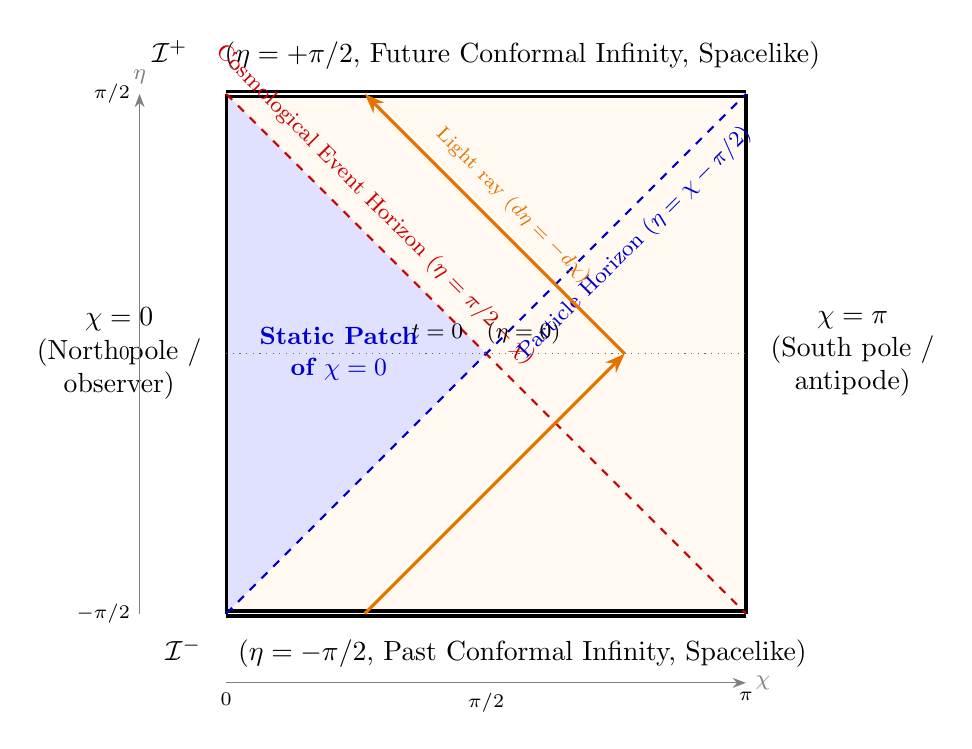
\begin{tikzpicture}[scale=2.2]
  % Coordinates of the square
  \coordinate (Im_left) at (0,-1.5);
  \coordinate (Im_right) at (3,-1.5);
  \coordinate (Ip_left) at (0,1.5);
  \coordinate (Ip_right) at (3,1.5);
  \coordinate (Center) at (1.5,0);
  
  % Shading
  \fill[orange!5] (0,-1.5) -- (3,-1.5) -- (3,1.5) -- (0,1.5) -- cycle;
  \fill[blue!12] (Im_left) -- (1.5,0) -- (Ip_left) -- cycle;

  % Boundaries
  % I- and I+ (spacelike boundaries, drawn with double lines)
  \draw[very thick, double, draw=black] (Im_left) -- node[below=5pt] {$\mathcal{I}^-$ \quad ($\eta = -\pi/2$, Past Conformal Infinity, Spacelike)} (Im_right);
  \draw[very thick, double, draw=black] (Ip_left) -- node[above=5pt] {$\mathcal{I}^+$ \quad ($\eta = +\pi/2$, Future Conformal Infinity, Spacelike)} (Ip_right);
  
  % Timelike poles (chi = 0 and chi = pi)
  \draw[very thick, draw=black] (Im_left) -- node[left=5pt, align=center] {$\chi = 0$\\ (North pole /\\ observer)} (Ip_left);
  \draw[very thick, draw=black] (Im_right) -- node[right=5pt, align=center] {$\chi = \pi$\\ (South pole /\\ antipode)} (Ip_right);
  
  % Horizons (45 degrees)
  \draw[thick, red!80!black, dashed] (Ip_left) -- node[pos=0.25, above=2pt, sloped, font=\footnotesize] {Cosmological Event Horizon ($\eta = \pi/2 - \chi$)} (Im_right);
  \draw[thick, blue!80!black, dashed] (Im_left) -- node[pos=0.75, below=2pt, sloped, font=\footnotesize] {Particle Horizon ($\eta = \chi - \pi/2$)} (Ip_right);
  
  % Light rays (45 degrees)
  \draw[line width=1.1pt, orange!90!black, -{Stealth[length=2.5mm]}] (0.8,-1.5) -- (2.3,0);
  \draw[line width=1.1pt, orange!90!black, -{Stealth[length=2.5mm]}] (2.3,0) -- node[pos=0.5, above=2pt, sloped, font=\scriptsize] {Light ray ($d\eta = -d\chi$)} (0.8,1.5);
  
  % Constant time slices (t = 0 / eta = 0)
  \draw[thin, dotted, gray!80!black] (0,0) -- node[above, font=\footnotesize, text=black] {$t = 0 \quad (\eta = 0)$} (3,0);
  
  % Static patch label
  \node[blue!80!black, align=center, font=\small\bfseries] at (0.65,0) {Static Patch\\ of $\chi = 0$};
  
  % Axes indication
  \draw[-{Stealth}, gray] (-0.5,-1.5) -- (-0.5,1.5) node[above, font=\footnotesize] {$\eta$};
  \node[left, font=\scriptsize] at (-0.5,-1.5) {$-\pi/2$};
  \node[left, font=\scriptsize] at (-0.5,0) {$0$};
  \node[left, font=\scriptsize] at (-0.5,1.5) {$\pi/2$};

  \draw[-{Stealth}, gray] (0,-1.9) -- (3,-1.9) node[right, font=\footnotesize] {$\chi$};
  \node[below, font=\scriptsize] at (0,-1.9) {$0$};
  \node[below, font=\scriptsize] at (1.5,-1.9) {$\pi/2$};
  \node[below, font=\scriptsize] at (3,-1.9) {$\pi$};
\end{tikzpicture}
\caption{Penrose diagram for de Sitter spacetime in global coordinates $(\eta, \chi)$. Light rays travel at $\pm 45^\circ$. Conformal infinities $\mathcal{I}^\pm$ are horizontal spacelike surfaces, and the shaded triangle represents the static causal diamond accessible to an observer at $\chi = 0$.}
\label{fig:penrose_ds}
\end{figure}

% =========================================================================
% QUESTION 5
% =========================================================================
\ques{6}{%
The linearised Einstein equation is
\be
- \frac{1}{2} \partial^\rho\partial_\rho \bh_{\mu\nu} + \partial^\rho \ partial_{(\mu} \bh_{\nu)\rho}
- \frac{1}{2} \eta_{\mu\nu} \partial^\rho \partial^\sigma \bh_{\rho\sigma} = 8 \pi G T_{\mu\nu} \,,
\label{eq:lin_einstein_q}
\ee
when written in terms of $\bh_{\mu\nu} = h_{\mu\nu} - \frac{1}{2} h \eta_{\mu\nu}$. 

\begin{enumerate}[label=\alph*)]
\item (\emph{1 point}) By making an appropriate gauge choice, explain why the linearised Einstein equation leads to \emph{gravitational waves}.
\item (\emph{2 point}) Consider an experiment involving two freely falling test particles, arranged so that one is at spatial position $x^i = (0,0,0)$ and the other at spatial position $x^i=(L_x,0,0)$.
Suppose a gravitational wave travelling along the $z$-axis passes through the laboratory, corresponding to the following metric perturbation:
\be
h_{\mu\nu} = \begin{pmatrix}
0 & 0 & 0 & 0 \\
0 & h_{+}(t-z) & 0 & 0 \\
0 & 0 & - h_{+}(t-z) & 0 \\
0 & 0 & 0 & 0
\end{pmatrix} \,.
\label{eq:plus_pol}
\ee
Show that the proper distance between the test particles is given by: 
\be
\Delta s \approx L_x \left( 1 + \frac{1}{2} h_{+}(t) \right) \,.
\ee
If a third test particle is introduced at $x^i=(0,L_y,0)$ show that the proper distance between it and the particle at the origin is
\be
\Delta s \approx L_y \left( 1 - \frac{1}{2} h_{+}(t) \right) \,.
\ee
\item (\emph{3 points}) Consider a binary system consisting of two massive bodies in a circular orbit, which are emitting gravitational waves.
Explain \emph{qualitatively} what happens to the system, and sketch the corresponding gravitational wave signal which would be observed by a detector such as LIGO.
You should mention the following terms: \emph{inspiral}, \emph{merger}, \emph{ringdown}, explain how the interferometer detects a wave such as that described in part b), and connect the features of the signal to the physics of the binary pair. 
\end{enumerate}
}

\subsection*{Part a) Gauge Choice and Gravitational Waves}

The metric of a weakly perturbed flat spacetime is $g_{\mu\nu} = \eta_{\mu\nu} + h_{\mu\nu}$ with $|h_{\mu\nu}| \ll 1$.
Under an infinitesimal coordinate transformation (gauge transformation) $x^\mu \to x'^\mu = x^\mu - \xi^\mu(x)$ with $|\partial_\mu \xi_\nu| \sim \mathcal{O}(h)$, the metric perturbation transforms as:
\be
h_{\mu\nu} \to h'_{\mu\nu} = h_{\mu\nu} + \partial_\mu \xi_\nu + \partial_\nu \xi_\mu \,.
\ee
Taking the trace with $\eta^{\mu\nu}$, the trace $h = \eta^{\mu\nu} h_{\mu\nu}$ transforms as:
\be
h \to h' = h + 2 \partial_\rho \xi^\rho \,.
\ee
The trace-reversed metric perturbation is defined by $\bar h_{\mu\nu} \equiv h_{\mu\nu} - \frac{1}{2} h \eta_{\mu\nu}$. Under the gauge transformation, it transforms as:
\be
\bar h_{\mu\nu} \to \bar h'_{\mu\nu} = \bar h_{\mu\nu} + \partial_\mu \xi_\nu + \partial_\nu \xi_\mu - \eta_{\mu\nu} \partial_\rho \xi^\rho \,.
\ee
Taking the 4-divergence with respect to $\partial^\mu$:
\be
\partial^\mu \bar h'_{\mu\nu} = \partial^\mu \bar h_{\mu\nu} + \partial^\mu \partial_\mu \xi_\nu + \partial^\mu \partial_\nu \xi_\mu - \partial_\nu \partial_\rho \xi^\rho = \partial^\mu \bar h_{\mu\nu} + \Box \xi_\nu \,,
\ee
where $\Box \equiv \partial^\rho \partial_\rho = -\frac{\partial^2}{\partial t^2} + \nabla^2$ is the flat-space d'Alembertian operator.
By choosing a gauge vector $\xi_\nu$ that satisfies the inhomogeneous wave equation $\Box \xi_\nu = - \partial^\mu \bar h_{\mu\nu}$ (which always possesses solutions), we can set $\partial^\mu \bar h'_{\mu\nu} = 0$.
This choice is the \textbf{Lorenz gauge condition} (also known as the de Donder, Hilbert, or harmonic gauge):
\be
\mathbf{\partial^\mu \bar h_{\mu\nu} = 0} \,.
\label{eq:lorenz_gauge}
\ee
Applying the Lorenz gauge condition \eqref{eq:lorenz_gauge} to the linearized Einstein equation \eqref{eq:lin_einstein_q}:
\begin{align}
\partial^\rho \partial_{(\mu} \bar h_{\nu)\rho} &= \frac{1}{2} \partial_\mu \left( \partial^\rho \bar h_{\nu\rho} \right) + \frac{1}{2} \partial_\nu \left( \partial^\rho \bar h_{\mu\rho} \right) = 0 \,, \\
\partial^\rho \partial^\sigma \bar h_{\rho\sigma} &= \partial^\rho \left( \partial^\sigma \bar h_{\rho\sigma} \right) = 0 \,.
\end{align}
Hence, the second and third terms in \eqref{eq:lin_einstein_q} vanish identically! The linearized field equation simplifies to:
\be
- \frac{1}{2} \Box \bar h_{\mu\nu} = 8\pi G T_{\mu\nu} \implies \mathbf{\Box \bar h_{\mu\nu} = - 16\pi G T_{\mu\nu}} \,.
\ee
In vacuum (far away from any matter sources, where $T_{\mu\nu} = 0$):
\be
\Box \bar h_{\mu\nu} = 0 \iff \left( - \frac{\partial^2}{\partial t^2} + \nabla^2 \right) \bar h_{\mu\nu} = 0 \,.
\label{eq:gw_wave_eq}
\ee
Equation \eqref{eq:gw_wave_eq} is the classical relativistic \textbf{wave equation} in four dimensions. It admits plane-wave solutions of the form:
\be
\bar h_{\mu\nu}(x) = A_{\mu\nu} e^{i k_\rho x^\rho} \,, \quad \text{with} \quad k^\rho k_\rho = 0 \implies \omega^2 = c^2 |\vec k|^2 \,.
\ee
This proves that disturbances in the gravitational field propagate through spacetime at the speed of light ($c=1$) as transverse, propagating ripples in the fabric of spacetime---known as \textbf{gravitational waves}.

\subsection*{Part b) Proper Distance Between Test Particles}

We are given the metric perturbation propagating along the $z$-axis in the transverse-traceless (TT) gauge:
\be
h_{\mu\nu} = \begin{pmatrix}
0 & 0 & 0 & 0 \\
0 & h_{+}(t-z) & 0 & 0 \\
0 & 0 & - h_{+}(t-z) & 0 \\
0 & 0 & 0 & 0
\end{pmatrix} \,.
\ee
The complete spacetime line element is $g_{\mu\nu} = \eta_{\mu\nu} + h_{\mu\nu}$, where $\eta_{\mu\nu} = \text{diag}(-1, +1, +1, +1)$:
\be
ds^2 = - dt^2 + \left[ 1 + h_+(t-z) \right] dx^2 + \left[ 1 - h_+(t-z) \right] dy^2 + dz^2 \,.
\label{eq:tt_line_element}
\ee

\paragraph{1. Coordinate Motion of Test Particles:}
First, we verify that freely falling test particles initially at rest remain at fixed spatial coordinates. 
The geodesic equation for a particle with 4-velocity $u^\mu = \frac{dx^\mu}{d\tau}$ is:
\be
\frac{du^\mu}{d\tau} + \Gamma^\mu_{\alpha\beta} u^\alpha u^\beta = 0 \,.
\ee
For a particle initially at rest, its 4-velocity is $u^\alpha = (1, 0, 0, 0)$. The initial acceleration is:
\be
\left. \frac{du^\mu}{d\tau} \right|_{\tau=0} = - \Gamma^\mu_{00} \,.
\ee
In linearized gravity, the Christoffel symbol components $\Gamma^\mu_{00}$ are:
\be
\Gamma^\mu_{00} = \frac{1}{2} \eta^{\mu\rho} \left( \partial_0 h_{\rho 0} + \partial_0 h_{0\rho} - \partial_\rho h_{00} \right) \,.
\ee
Since $h_{0\rho} = 0$ for all $\rho \in \{0,1,2,3\}$ in the TT gauge, all derivatives of $h_{0\rho}$ vanish identically:
\be
\Gamma^\mu_{00} = 0 \implies \left. \frac{du^\mu}{d\tau} \right|_{\tau=0} = 0 \,.
\ee
Consequently, particles initially at rest experience zero coordinate acceleration and remain permanently at their initial spatial coordinate positions:
\begin{align}
\text{Particle 1:} \quad &x_1^i = (0, 0, 0) \,, \\
\text{Particle 2:} \quad &x_2^i = (L_x, 0, 0) \,, \\
\text{Particle 3:} \quad &x_3^i = (0, L_y, 0) \,.
\end{align}

\paragraph{2. Proper Distance between Particle 1 and Particle 2 (along the $x$-axis):}
To find the physical proper distance $\Delta s$ between Particle 1 and Particle 2 at an instant of coordinate time $t$, we compute the spacelike line integral along the spatial path connecting them at constant $t$, $y = 0$, and $z = 0$.
Along this path:
\be
dt = 0 \,, \quad dy = 0 \,, \quad dz = 0 \,, \quad x \in [0, L_x] \,.
\ee
Since $z = 0$ everywhere along this trajectory, the argument of the wave is $t - z = t - 0 = t$.
The line element \eqref{eq:tt_line_element} reduces to:
\be
ds^2 = g_{xx} dx^2 = \left[ 1 + h_+(t) \right] dx^2 \,.
\ee
The proper distance is given by the integral:
\be
\Delta s = \int_0^{L_x} \sqrt{g_{xx}} \, dx = \int_0^{L_x} \sqrt{1 + h_+(t)} \, dx \,.
\ee
Because the metric perturbation is very weak, $|h_+(t)| \ll 1$. Applying the first-order Taylor/binomial expansion:
\be
\sqrt{1 + h_+(t)} = \left( 1 + h_+(t) \right)^{1/2} = 1 + \frac{1}{2} h_+(t) + \mathcal{O}(h_+^2) \,.
\ee
Since $h_+(t)$ does not depend on the spatial coordinate $x$, it factors out of the integral:
\be
\Delta s \approx \int_0^{L_x} \left( 1 + \frac{1}{2} h_+(t) \right) dx = \left( 1 + \frac{1}{2} h_+(t) \right) \int_0^{L_x} dx \,.
\ee
Evaluating the integral gives the desired result:
\be
\mathbf{\Delta s \approx L_x \left( 1 + \frac{1}{2} h_{+}(t) \right)} \,.
\ee

\paragraph{3. Proper Distance between Particle 1 and Particle 3 (along the $y$-axis):}
Now consider the third test particle located at $(0, L_y, 0)$. At the same instant of coordinate time $t$, the spatial path connecting Particle 1 at $(0,0,0)$ to Particle 3 at $(0,L_y,0)$ has:
\be
dt = 0 \,, \quad dx = 0 \,, \quad dz = 0 \,, \quad y \in [0, L_y] \,.
\ee
Along this path, $z = 0$, so $h_+(t - z) = h_+(t)$.
The line element \eqref{eq:tt_line_element} reduces to:
\be
ds^2 = g_{yy} dy^2 = \left[ 1 - h_+(t) \right] dy^2 \,.
\ee
The proper distance is:
\be
\Delta s = \int_0^{L_y} \sqrt{g_{yy}} \, dy = \int_0^{L_y} \sqrt{1 - h_+(t)} \, dy \,.
\ee
Using the first-order binomial expansion for $|h_+(t)| \ll 1$:
\be
\sqrt{1 - h_+(t)} = \left( 1 - h_+(t) \right)^{1/2} = 1 - \frac{1}{2} h_+(t) + \mathcal{O}(h_+^2) \,.
\ee
Integrating over $y$ from $0$ to $L_y$:
\be
\Delta s \approx \int_0^{L_y} \left( 1 - \frac{1}{2} h_+(t) \right) dy = \left( 1 - \frac{1}{2} h_+(t) \right) \int_0^{L_y} dy \,.
\ee
Evaluating the integral yields:
\be
\mathbf{\Delta s \approx L_y \left( 1 - \frac{1}{2} h_{+}(t) \right)} \,.
\ee
\emph{Physical Interpretation:} As the gravitational wave passes, when the proper distance along the $x$-axis expands by $+\frac{1}{2} L_x h_+(t)$, the proper distance along the orthogonal $y$-axis simultaneously contracts by $-\frac{1}{2} L_y h_+(t)$. This differential quadrupolar strain is the signature of the plus ($+$) polarization of gravitational radiation.

\subsection*{Part c) Binary System, Interferometer Detection, and Signal Features}

\paragraph{1. Qualitative Physics of a Coalescing Binary System:}
Consider a binary system composed of two massive compact objects (such as two black holes or neutron stars) with masses $m_1$ and $m_2$ in a circular orbit of separation $r$ with orbital frequency $\omega_{\text{orb}}$.
According to general relativity, a time-dependent mass quadrupole moment radiates energy in the form of gravitational waves. The total power radiated is given by the Einstein quadrupole formula:
\be
P = - \frac{dE_{\text{orbit}}}{dt} = \frac{32 G}{5 c^5} \mu^2 r^4 \omega_{\text{orb}}^6 > 0 \,,
\label{eq:quadrupole_power}
\ee
where $\mu = \frac{m_1 m_2}{m_1 + m_2}$ is the reduced mass, and the total mass is $M = m_1 + m_2$.
By Kepler's third law, $\omega_{\text{orb}}^2 = \frac{GM}{r^3}$. The mechanical energy of the circular orbit is $E_{\text{orbit}} = - \frac{G m_1 m_2}{2r} < 0$. 

The continuous emission of gravitational waves drains orbital energy and angular momentum from the system. As energy is lost:
\begin{enumerate}
    \item The orbital separation $r(t)$ must decrease (the orbit shrinks).
    \item By Kepler's third law, as $r$ decreases, the orbital frequency $\omega_{\text{orb}} \propto r^{-3/2}$ must increase.
    \item The frequency of the emitted gravitational waves is twice the orbital frequency: $f_{\text{GW}} = 2 f_{\text{orb}} = \frac{\omega_{\text{orb}}}{\pi}$.
\end{enumerate}
This feedback loop drives the system through three distinct physical stages:

\begin{itemize}
    \item \textbf{1. Inspiral Phase:}
    In this stage, the two bodies orbit each other with adiabatically shrinking separation. Because the separation $r$ decreases, both the frequency $f_{\text{GW}}(t)$ and the amplitude $h(t)$ of the emitted gravitational waves steadily increase with time:
    \be
    f_{\text{GW}}(t) \propto (t_{\text{merger}} - t)^{-3/8} \,, \qquad h(t) \propto \frac{\mathcal{M}^{5/3} f_{\text{GW}}^{2/3}}{D_L} \propto (t_{\text{merger}} - t)^{-1/4} \,,
    \ee
    where $\mathcal{M} = \frac{(m_1 m_2)^{3/5}}{(m_1 + m_2)^{1/5}}$ is the \emph{chirp mass}, and $D_L$ is the luminosity distance. This produces the distinctive \textbf{chirp} signal---a sinusoidal waveform sweeping upward in both pitch (frequency) and volume (amplitude). This regime is accurately modeled by post-Newtonian (PN) analytic expansions.

    \item \textbf{2. Merger Phase:}
    As the orbital separation decreases to the Innermost Stable Circular Orbit (ISCO), stable circular motion ceases. The two objects plunge toward each other at relativistic velocities ($v \sim 0.5c$) and violently coalesce into a single, highly deformed, highly dynamical remnant black hole. In this phase, the spacetime curvature is extreme and the field equations are fully non-linear, requiring numerical relativity simulations. The gravitational wave strain reaches its absolute \textbf{peak amplitude} during the merger.

    \item \textbf{3. Ringdown Phase:}
    The newly formed, distorted remnant black hole sheds its non-axisymmetric multipole deformations by emitting gravitational waves to settle down into a stationary Kerr black hole. The signal during ringdown is described by black hole perturbation theory and consists of a superposition of damped sinusoids called \textbf{quasi-normal modes (QNMs)}:
    \be
    h(t) = A_0 \, e^{-t/\tau} \cos(\omega_{\text{QNM}} t + \phi_0) \,.
    \ee
    By the black hole \emph{no-hair theorem}, the central frequency $\omega_{\text{QNM}}$ and the damping timescale $\tau$ depend exclusively on the final black hole's mass $M_f$ and spin parameter $a_f = J_f / M_f$.
\end{itemize}

\paragraph{2. How an Interferometer (such as LIGO) Detects Gravitational Waves:}
A gravitational wave detector like LIGO is a large-scale Michelson laser interferometer with two orthogonal arms oriented along the $x$- and $y$-axes, each of nominal arm length $L_x = L_y = L \approx 4\text{ km}$.
The mirrors (test masses) at the ends of the arms and the central beam splitter are suspended as pendulums, making them essentially freely falling in the horizontal plane above their resonant frequency.

When a gravitational wave with polarization $h_+(t)$ propagating along the $z$-axis strikes the detector perpendicularly, the calculations from part b) show that:
\be
\Delta L_x(t) \approx \frac{1}{2} L h_+(t) \,, \qquad \Delta L_y(t) \approx - \frac{1}{2} L h_+(t) \,.
\ee
The differential change in the arm lengths is therefore:
\be
\Delta L(t) = \Delta L_x(t) - \Delta L_y(t) \approx L h_+(t) \,.
\ee
Laser light of wavelength $\lambda$ is split at the beam splitter, travels down each arm, bounces off the end mirrors, and returns to recombine at the beam splitter. The round-trip travel time difference $\Delta \tau = \frac{2 \Delta L(t)}{c}$ introduces an optical phase shift between the two returning laser beams:
\be
\Delta \Phi(t) = \frac{2\pi c}{\lambda} \Delta \tau = \frac{4\pi}{\lambda} \Delta L(t) = \frac{4\pi L}{\lambda} h_+(t) \,.
\ee
The interferometer is tuned so that in the absence of a gravitational wave, the recombining beams interfere destructively at the output port (the ``dark fringe''). When the gravitational wave passes, the differential arm length change $\Delta L(t)$ shifts the optical phase, allowing a small amount of light to escape to the photodetector:
\be
P_{\text{out}}(t) \propto \sin^2\left(\frac{\Delta \Phi(t)}{2}\right) \approx \frac{1}{4} \left(\frac{4\pi L}{\lambda}\right)^2 h_+^2(t) \,.
\ee
Using RF modulation and homodyne readout techniques, the output signal is made linearly proportional to $h_+(t)$. By utilizing Fabry-P\'erot resonant cavities to increase the effective arm length and power recycling mirrors, LIGO achieves sensitivity capable of measuring differential displacements as small as $\Delta L \sim 10^{-19}\text{ m}$, corresponding to strains $h \sim 10^{-21}$!

\paragraph{3. Connecting Signal Features to Binary Physics:}
\begin{itemize}
    \item \textbf{Chirp Rate and Chirp Mass:} The rate at which the gravitational wave frequency increases, $\dot f_{\text{GW}} = \frac{96}{5} \pi^{8/3} \left( \frac{G \mathcal{M}}{c^3} \right)^{5/3} f_{\text{GW}}^{11/3}$, depends solely on the chirp mass $\mathcal{M} = \frac{(m_1 m_2)^{3/5}}{(m_1+m_2)^{1/5}}$. Measuring $\dot f_{\text{GW}}(t)$ allows an extraordinarily precise determination of $\mathcal{M}$.
    \item \textbf{Amplitude and Luminosity Distance:} Combined with the chirp mass, the measured wave amplitude $h \propto \frac{\mathcal{M}^{5/3} f^{2/3}}{D_L}$ provides a direct measurement of the luminosity distance $D_L$ to the source without needing a cosmic distance ladder (making binary coalescences ``standard sirens'').
    \item \textbf{Peak Frequency and Total Mass:} The frequency at which the amplitude peaks corresponds to the transition from inspiral to plunge/merger at the ISCO ($f_{\text{ISCO}} \approx \frac{c^3}{6^{3/2} \pi G M}$), directly constraining the total mass $M = m_1 + m_2$.
    \item \textbf{Ringdown Frequency and Damping:} Measuring the damped sinusoidal frequency $\omega_{\text{QNM}}$ and decay time $\tau$ provides an independent measurement of the mass $M_f$ and dimensionless spin parameter $a_f$ of the final remnant black hole, providing a direct test of Hawking's area theorem and the Kerr nature of black holes in general relativity.
\end{itemize}

\begin{figure}[htbp]
\centering
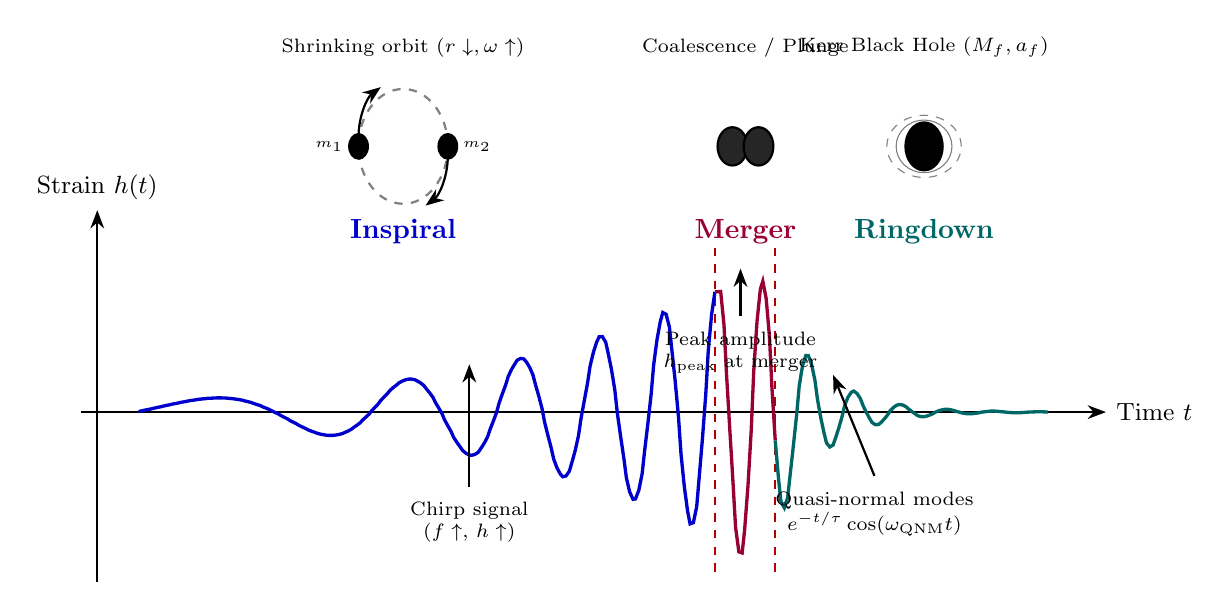
\begin{tikzpicture}[xscale=1.05, yscale=1.35]
  % Grid / Axes
  \draw[-{Stealth}, thick] (-0.2,0) -- (12.2,0) node[right, font=\small] {Time $t$};
  \draw[-{Stealth}, thick] (0,-1.6) -- (0,1.9) node[above, font=\small] {Strain $h(t)$};
  
  % Phase boundaries
  \draw[dashed, red!70!black, thick] (7.47,-1.5) -- (7.47,1.6);
  \draw[dashed, red!70!black, thick] (8.20,-1.5) -- (8.20,1.6);
  
  % Phase labels
  \node[font=\bfseries\normalsize, text=blue!80!black] at (3.7, 1.7) {Inspiral};
  \node[font=\bfseries\normalsize, text=purple!80!black] at (7.84, 1.7) {Merger};
  \node[font=\bfseries\normalsize, text=teal!80!black] at (10.0, 1.7) {Ringdown};
  
  % Binary Orbit Sketches
  % Inspiral orbit cartoon
  \begin{scope}[shift={(3.7,2.5)}, scale=0.45]
    \draw[thick, gray, dashed] (0,0) circle (1.2);
    \fill[black] (-1.2,0) circle (0.28) node[left=2pt, font=\tiny] {$m_1$};
    \fill[black] (1.2,0) circle (0.28) node[right=2pt, font=\tiny] {$m_2$};
    \draw[-{Stealth}, thick] (-1.2,0.2) arc (180:120:1.2);
    \draw[-{Stealth}, thick] (1.2,-0.2) arc (0:-60:1.2);
    \node[above=8pt, font=\scriptsize] at (0,1.2) {Shrinking orbit ($r \downarrow, \omega \uparrow$)};
  \end{scope}
  
  % Merger cartoon
  \begin{scope}[shift={(7.84,2.5)}, scale=0.45]
    \draw[thick, fill=black!85] (-0.35,0) circle (0.4);
    \draw[thick, fill=black!85] (0.35,0) circle (0.4);
    \node[above=8pt, font=\scriptsize] at (0,1.2) {Coalescence / Plunge};
  \end{scope}
  
  % Ringdown cartoon
  \begin{scope}[shift={(10.0,2.5)}, scale=0.45]
    \draw[thick, fill=black] (0,0) circle (0.5);
    \draw[thin, gray] (0,0) ellipse (0.75 and 0.55);
    \draw[thin, gray, dashed] (0,0) ellipse (1.0 and 0.65);
    \node[above=8pt, font=\scriptsize] at (0,1.2) {Kerr Black Hole ($M_f, a_f$)};
  \end{scope}

  % Waveform - Inspiral (Continuous coordinates)
  \draw[very thick, blue!80!black] plot coordinates {
    (0.50,0.006) (0.54,0.012) (0.57,0.018) (0.61,0.024) (0.65,0.030) (0.68,0.036) (0.72,0.043) (0.76,0.049) (0.79,0.055) (0.83,0.062) (0.87,0.068) (0.90,0.074) (0.94,0.080) (0.98,0.086) (1.01,0.092) (1.05,0.097) (1.09,0.103) (1.12,0.108) (1.16,0.112) (1.20,0.117) (1.23,0.121) (1.27,0.124) (1.31,0.127) (1.34,0.130) (1.38,0.131) (1.42,0.133) (1.45,0.134) (1.49,0.134) (1.53,0.133) (1.56,0.132) (1.60,0.129) (1.64,0.126) (1.67,0.123) (1.71,0.118) (1.75,0.113) (1.78,0.106) (1.82,0.099) (1.86,0.091) (1.89,0.082) (1.93,0.072) (1.97,0.062) (2.00,0.050) (2.04,0.038) (2.08,0.025) (2.11,0.012) (2.15,-0.003) (2.19,-0.017) (2.22,-0.032) (2.26,-0.048) (2.30,-0.063) (2.33,-0.079) (2.37,-0.095) (2.41,-0.110) (2.44,-0.125) (2.48,-0.140) (2.52,-0.154) (2.55,-0.167) (2.59,-0.179) (2.63,-0.190) (2.66,-0.199) (2.70,-0.207) (2.74,-0.213) (2.77,-0.217) (2.81,-0.219) (2.85,-0.219) (2.88,-0.216) (2.92,-0.211) (2.96,-0.203) (2.99,-0.193) (3.03,-0.179) (3.07,-0.163) (3.10,-0.145) (3.14,-0.124) (3.18,-0.100) (3.21,-0.074) (3.25,-0.046) (3.29,-0.017) (3.32,0.014) (3.36,0.046) (3.40,0.079) (3.43,0.111) (3.47,0.143) (3.51,0.174) (3.54,0.204) (3.58,0.231) (3.62,0.255) (3.65,0.276) (3.69,0.292) (3.73,0.304) (3.76,0.310) (3.80,0.311) (3.84,0.305) (3.87,0.293) (3.91,0.275) (3.95,0.250) (3.98,0.219) (4.02,0.182) (4.06,0.139) (4.09,0.091) (4.13,0.039) (4.17,-0.015) (4.20,-0.072) (4.24,-0.128) (4.28,-0.184) (4.31,-0.237) (4.35,-0.285) (4.39,-0.328) (4.42,-0.362) (4.46,-0.388) (4.50,-0.403) (4.53,-0.406) (4.57,-0.397) (4.61,-0.376) (4.64,-0.341) (4.68,-0.293) (4.72,-0.234) (4.75,-0.164) (4.79,-0.086) (4.83,-0.002) (4.86,0.085) (4.90,0.173) (4.94,0.257) (4.97,0.334) (5.01,0.401) (5.05,0.453) (5.08,0.489) (5.12,0.505) (5.16,0.500) (5.19,0.472) (5.23,0.421) (5.27,0.349) (5.30,0.258) (5.34,0.151) (5.38,0.032) (5.41,-0.093) (5.45,-0.218) (5.49,-0.336) (5.52,-0.440) (5.56,-0.524) (5.60,-0.582) (5.63,-0.608) (5.67,-0.600) (5.71,-0.555) (5.74,-0.475) (5.78,-0.363) (5.82,-0.223) (5.85,-0.064) (5.89,0.106) (5.93,0.274) (5.96,0.430) (6.00,0.561) (6.04,0.658) (6.07,0.709) (6.11,0.710) (6.15,0.657) (6.18,0.551) (6.22,0.398) (6.26,0.207) (6.29,-0.008) (6.33,-0.229) (6.37,-0.440) (6.40,-0.620) (6.44,-0.752) (6.48,-0.820) (6.51,-0.816) (6.55,-0.735) (6.59,-0.581) (6.62,-0.365) (6.66,-0.105) (6.70,0.175) (6.73,0.447) (6.77,0.682) (6.81,0.853) (6.84,0.937) (6.88,0.921) (6.92,0.800) (6.95,0.583) (6.99,0.291) (7.03,-0.047) (7.06,-0.391) (7.10,-0.699) (7.14,-0.931) (7.17,-1.051) (7.21,-1.040) (7.25,-0.890) (7.28,-0.615) (7.32,-0.246) (7.36,0.170) (7.39,0.577) (7.43,0.915) (7.47,1.131)
  };
    
  % Waveform - Merger (Continuous coordinates)
  \draw[very thick, purple!80!black] plot coordinates {
    (7.47,1.131) (7.54,1.135) (7.58,0.823) (7.61,0.369) (7.65,-0.158) (7.69,-0.671) (7.72,-1.081) (7.76,-1.314) (7.80,-1.325) (7.83,-1.106) (7.87,-0.696) (7.91,-0.166) (7.94,0.386) (7.98,0.856) (8.02,1.156) (8.05,1.231) (8.09,1.071) (8.13,0.712) (8.16,0.233) (8.20,-0.267)
  };
    
  % Waveform - Ringdown (Continuous coordinates)
  \draw[very thick, teal!80!black] plot coordinates {
    (8.20,-0.267) (8.24,-0.629) (8.27,-0.846) (8.31,-0.900) (8.35,-0.805) (8.38,-0.592) (8.42,-0.311) (8.46,-0.016) (8.49,0.246) (8.53,0.436) (8.57,0.533) (8.60,0.533) (8.64,0.447) (8.68,0.301) (8.71,0.125) (8.75,-0.050) (8.79,-0.195) (8.82,-0.290) (8.86,-0.328) (8.90,-0.309) (8.93,-0.242) (8.97,-0.146) (9.01,-0.037) (9.04,0.063) (9.08,0.141) (9.12,0.187) (9.15,0.198) (9.19,0.175) (9.23,0.127) (9.26,0.065) (9.30,0.000) (9.34,-0.057) (9.37,-0.097) (9.41,-0.118) (9.45,-0.117) (9.48,-0.097) (9.52,-0.064) (9.56,-0.025) (9.59,0.013) (9.63,0.044) (9.67,0.065) (9.70,0.072) (9.74,0.067) (9.78,0.052) (9.81,0.031) (9.85,0.007) (9.89,-0.015) (9.92,-0.032) (9.96,-0.042) (10.00,-0.043) (10.03,-0.038) (10.07,-0.027) (10.11,-0.014) (10.14,0.001) (10.18,0.013) (10.22,0.022) (10.25,0.026) (10.29,0.026) (10.33,0.021) (10.36,0.014) (10.40,0.005) (10.44,-0.003) (10.47,-0.010) (10.51,-0.014) (10.55,-0.016) (10.58,-0.015) (10.62,-0.011) (10.66,-0.007) (10.69,-0.001) (10.73,0.003) (10.77,0.007) (10.80,0.009) (10.84,0.010) (10.88,0.008) (10.91,0.006) (10.95,0.003) (10.99,-0.000) (11.02,-0.003) (11.06,-0.005) (11.10,-0.006) (11.13,-0.006) (11.17,-0.005) (11.21,-0.003) (11.24,-0.001) (11.28,0.001) (11.32,0.002) (11.35,0.003) (11.39,0.003) (11.43,0.003) (11.46,0.002) (11.50,0.001)
  };

  % Annotations on waveform
  \draw[{Stealth}-, thick] (7.78, 1.35) -- (7.78, 0.9) node[below=2pt, font=\scriptsize, align=center] {Peak amplitude\\ $h_{\text{peak}}$ at merger};
  \draw[{Stealth}-, thick] (4.5, 0.45) -- (4.5, -0.7) node[below=2pt, font=\scriptsize, align=center] {Chirp signal\\ ($f \uparrow$, $h \uparrow$)};
  \draw[{Stealth}-, thick] (8.9, 0.35) -- (9.4, -0.6) node[below=2pt, font=\scriptsize, align=center] {Quasi-normal modes\\ $e^{-t/\tau} \cos(\omega_{\text{QNM}} t)$};
\end{tikzpicture}
\caption{Schematic waveform of the gravitational wave strain $h(t)$ emitted during the coalescence of a binary compact system, demonstrating the three stages: (i) the \emph{inspiral} with increasing amplitude and frequency (the chirp), (ii) the violent \emph{merger} reaching maximum amplitude, and (iii) the exponentially damped \emph{ringdown} of quasi-normal modes settling into a stationary Kerr black hole.}
\label{fig:gw_chirp}
\end{figure}

\end{document}
